\documentclass[a4paper, 14pt]{article}
\usepackage[utf8]{inputenc}
\usepackage{hyperref}
\usepackage{nth}
\usepackage{graphicx}
\usepackage{listings}
\usepackage[square, numbers, comma, sort&compress]{natbib}
\date{\vspace{-5ex}}
\begin{document}
	\begin{center}
		Name : ANIRBAN MITRA \\
		ROLL N.O: 14EE10004
	\end{center}
	\begin{itemize}
		\item Number of SM : 16
		\item Cores Per SM: 128
		\item Warp Size : 32
		\item Shared Memory : 64Kb
	\end{itemize}
	\paragraph{Reduction}
	Reduction serves as an efficient data parallel primitive. Our main goal should be to efficiently process large arrays, to keep maximum number of multiprocessors on the GPU busy and such that each thread block reduces a portion of the array.

	The goal should be that at the block level , bring data in shared memory and the we should start adding in parallel. The amount of shared memory to be used is sent as a parameter in the kernel launch function. In reduction gradually fewer and fewer threads of a block participate.
	
	I have used two kernel launches to calculate the matrix sum. The first one is used to calculate the sum in each block and the next launch is to calculate the sum across the blocks. The requirement is that the blocksize taken should be a multiple of 4.
	\\
	The naive implementation faces the problem that highly divergent warps are very inefficient, and the modulo \% checking operator is very slow.

	\begin{figure}[h]
		\centering
		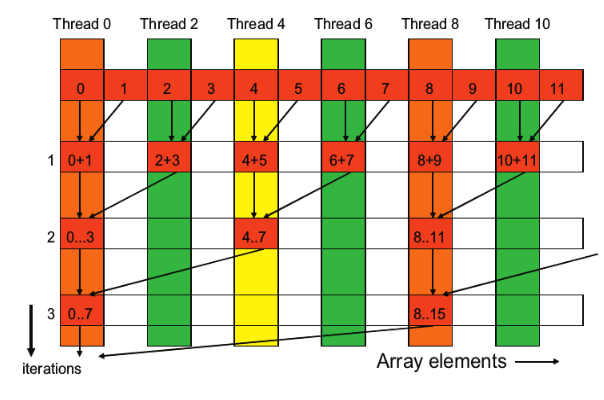
\includegraphics[scale=0.6]{naive.png}
		\label{fig:kgplogo}
	\end{figure}
	Iplementation:
		
	\begin{lstlisting}
	__global__ void ReduceRowMajor(int *g_idata, int *g_odata, int size) {
		unsigned int i = blockIdx.x*blockDim.x + threadIdx.x;	
		unsigned int tid = threadIdx.x;
		extern __shared__ int sdata[];
		sdata[tid] = 0;
		if(i < size)
		sdata[tid] = g_idata[i];
		__syncthreads();
		for(unsigned int s = 4; s < blockDim.x; s*=2) {
		if(tid%(2*s) == 0) {
			sdata[tid] += sdata[tid+s];
			sdata[tid+1] += sdata[tid+s+1];
			sdata[tid+2] += sdata[tid+s+2];
			sdata[tid+3] += sdata[tid+s+3];
		}	
		__syncthreads();
		}
		if(tid == 0) {
			g_odata[blockIdx.x*4] = sdata[0];
			g_odata[blockIdx.x*4+1] = sdata[1];
			g_odata[blockIdx.x*4+2] = sdata[2];
			g_odata[blockIdx.x*4+3] = sdata[3];
		}
	}
	
	\end{lstlisting}
	\par
	In the second optimization I just removed the divergent branch in the inner loop with strided index and non-divergent branch. It shows some speed up but can still further be improved.

	Another optimization can be using reversed loop and threadId-based indexing. This method serves a lot like binary search and each step half of the threads do the required work. 
	\par
	\begin{lstlisting}
	__global__ void ReduceRowMajor3(int *g_idata, int *g_odata, int size) {
		unsigned int i = blockIdx.x*blockDim.x + threadIdx.x;	
		unsigned int tid = threadIdx.x;
		extern __shared__ int sdata[];
		sdata[tid] = 0;
		if(i < size)
		sdata[tid] = g_idata[i];
		__syncthreads();
		for(unsigned int s = blockDim.x/2; s > 3; s/=2) {
			if(tid < s) {
				sdata[tid] += sdata[tid+s];
			}	
		__syncthreads();
		}
		if(tid == 0) {
			g_odata[blockIdx.x*4] = sdata[0];
			g_odata[blockIdx.x*4+1] = sdata[1];
			g_odata[blockIdx.x*4+2] = sdata[2];
			g_odata[blockIdx.x*4+3] = sdata[3];
		}
	}
	\end{lstlisting}
	But as the loop starts from $blockIdx.x/2$, half of the threads at the first itteration are all wasted.
	
	Optimized Technique: Using Unrolling

	As reduction proceeds , the number of active threads decreases and when $s <=32$ we only have one wrap left. Instructions are SIMD synchronous within a warp.
	
	This means when $s<=32$, there is no need of using $ $ $\_\_syncthreads()$ and also we do not need to check if $tid < s$.
	
	This saves useless work in all warps. Without unrolling all warps execute every itteration of the for loop and if statement.
	\\
	Implementation:
	\begin{lstlisting}
	__global__ void ReduceRowMajor5(int *g_idata, int *g_odata, int size) {
		unsigned int i = blockIdx.x*blockDim.x + threadIdx.x;	
		unsigned int tid = threadIdx.x;
		extern __shared__ int sdata[];
		sdata[tid] = 0;
		if(i < size)
		sdata[tid] = g_idata[i];
		__syncthreads();
		for(unsigned int s = blockDim.x/2; s >= 32; s/=2) {
		if(tid < s) {
			sdata[tid] += sdata[tid+s];
		}	
		__syncthreads();
		}
		if(tid < 32) {
		warpReduce(sdata, tid, size);
		}
		if(tid == 0) {
			g_odata[blockIdx.x*4] = sdata[0];
			g_odata[blockIdx.x*4+1] = sdata[1];
			g_odata[blockIdx.x*4+2] = sdata[2];
			g_odata[blockIdx.x*4+3] = sdata[3];
		}
	}
	
	__device__ void warpReduce(volatile int* sdata, int tid, int n) {
		if(tid + 32 < n)
		sdata[tid] += sdata[tid+32];
		if(tid + 16 < n)
		sdata[tid] += sdata[tid+16];
		if(tid + 8 < n)	
		sdata[tid] += sdata[tid+8];
		if(tid + 4 < n)	
		sdata[tid] += sdata[tid+4];
	}
	\end{lstlisting}
\end{document}